\documentclass{standalone}
\usepackage{tikz}
\usetikzlibrary{arrows,arrows.meta,positioning}
\usetikzlibrary{calc}
\usetikzlibrary{shapes.geometric}

\begin{document}
\begin{tikzpicture}[
            font={\sffamily \small},
            scale=1.,
            >=latex,
            transform shape,
            zoom/.style={line width=.5pt,shorten >=0pt,shorten <=0pt,densely dashed},
        ]
	
		\node[inner sep=0pt] (whitehead) at (-3.4,0.)
       {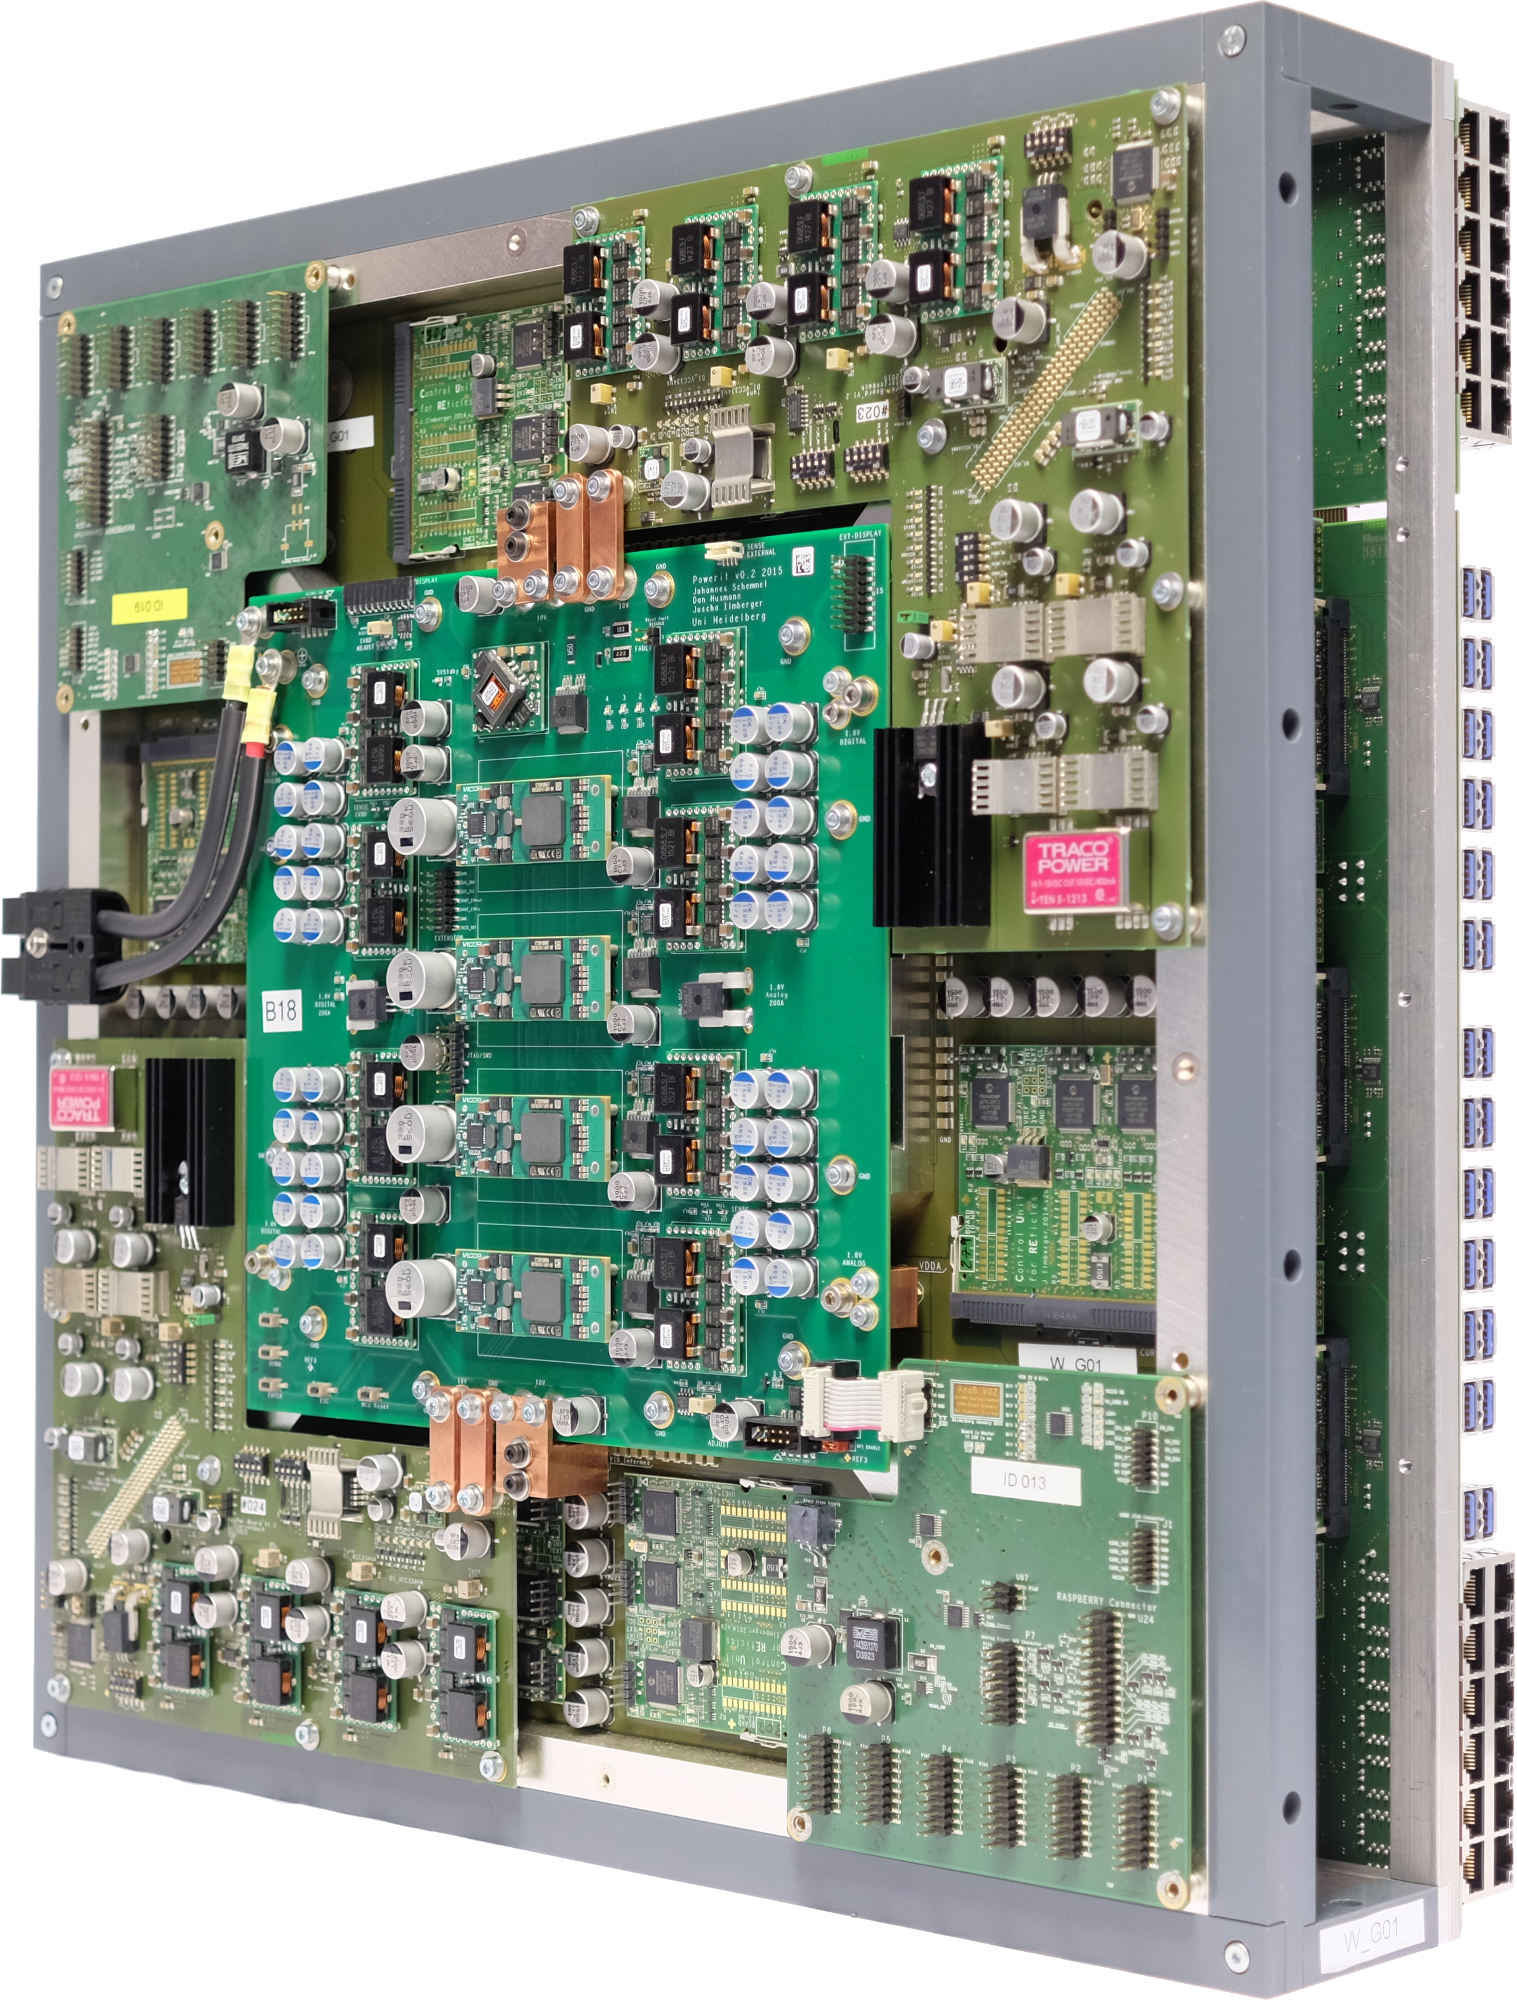
\includegraphics[width=.37\textwidth]{wmod}};
		 

	\pgfresetboundingbox
	\draw[use as bounding box,inner sep=0pt] node {\includegraphics[width=\textwidth]{figHardware}};
\end{tikzpicture}
\end{document}